\chapter{Redes Neuronales Totalmente Conectadas}

\section{Estructura}

\subsection{Neurona}
\subsection{Conexión entre capas}
\subsection{Función de activación}

RELU para capas intermedias, sigmoide para última capa.

\subsection{Función de error o pérdida}
% https://medium.com/mlearning-ai/understanding-loss-functions-for-classification-81c19ee72c2a

Como solo tenemos dos clases y estamos en clasificación binaria, usaremos Sigmoid Cross Entropy Loss.

\begin{gather}
   H(x) = - \frac{1}{N} \sum_{i=1}^{N}  [y_i * log( \hat{y}_i) + (1-y_i)*log(1-\hat{y_i})]
\end{gather}

y = etiqueta real \\
$\hat{y}$ = predicción 

\section{ForwardPropagation}
\section{Descenso del gradiente}
\section{BackPropagation}
\subsection{1 capa oculta}

\begin{figure}[H]
	\centering
	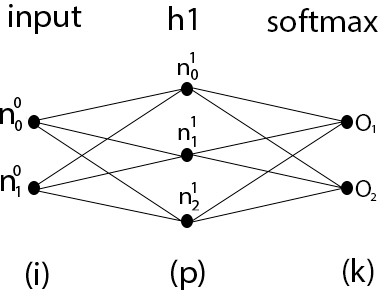
\includegraphics[scale=0.35]{imagenes/nn_1_capa.jpg}  
	\caption{Red Neuronal totalmente conectada con 1 capa oculta}
	\label{fig:nn_1_capa}
\end{figure}


\subsubsection{Capa output}

Sea la neurona $n$, se define como $n_{in}$ el valor de dicha neurona antes de aplicar sobre ella su función de activación asociada, y $n_{out}$ el obtenido tras aplicarla.
De esta forma, si la última capa es $\hat{y}$ y solo tiene una neurona, $\hat{y_{in}}$ y $\hat{y_{out}}$ corresponderán con los valores antes y después de aplicar la función de activación respectivamente.\\

De esta forma, la función de pérdida (2.1) se convierte en:

\begin{gather}
    H(x) = - \frac{1}{N} \sum_{i=1}^{N}  [y_i * log( \hat{y}_{out_i}) + (1-y_i)*log(1-\hat{y}_{out_i})]
\end{gather}

Para realizar el descenso del gradiente, se debe empezar calculando la derivada de la función de pérdida respecto a la predicción obtenida. Es decir, la derivada de la fórmula (2.2) respecto de las neuronas en la última capa de la red tras aplicar sus respectivas funciones de activación, que en este caso corresponde a $\hat{y}_{out}$. \\
Por simplicidad, podemos dividir esta derivada en 2 partes. \\
Parte izquierda:
\begin{gather}
	f(x) = A*B \\  
	f'(x) = AB' + A'B \\
	\frac{dy_i}{d\hat{y}_{out_i}} = 0 \\
	\frac{dlog(\hat{y}_{out_i} )}{d\hat{y}_{out_i}} = \frac{1}{\hat{y}_{out_i}} \\
	\frac{dy_i * log( \hat{y}_{out_i})}{d\hat{y}_{out_i}} = y_i*\frac{1}{\hat{y}_{out_i}} + 0*log(\hat{y}_{out_i} ) = \frac{y_i}{\hat{y}_{out_i}}
\end{gather}

Parte derecha:
\begin{gather}
	\frac{d(1-y_i)}{d\hat{y}_{out_i}} = 0\\
	\frac{dlog(1-\hat{y}_{out_i})}{d\hat{y}_{out_i}} = \frac{1}{1-\hat{y}_{out_i}} * (-1) \\
	\frac{d(1-y_i)*log(1-\hat{y}_{out_i})}{d\hat{y}_{out_i}} = (1-y_i)*\frac{1}{1-\hat{y}_{out_i}}*(-1) + 0* log(1-\hat{y}_{out_i}) \\
	\frac{d(1-y_i)*log(1-\hat{y}_{out_i})}{d\hat{y}_{out_i}} = -\frac{1-y_i}{1-\hat{y}_{out_i}}
\end{gather}

Finalmente, se obtiene: 
\begin{gather}
    \frac{dH(x)}{d\hat{y}_{out_i}} = - \frac{1}{N} \sum_{i=1}^{N}  [ \frac{y_i}{\hat{y}_{out_i}} - \frac{1-y_i}{1-\hat{y}_{out_i}} ]
\end{gather}

\subsubsection{Capa oculta h1}

\subsubsection{Capa input}